\chapter{背景と問題提起}
\label{chap:related_works}
% 本章では,Service Function Chaining (SFC),及びそれを実現する技術について解説する.
% SFC を実現するための技術は複数存在する.
% 本論文では,複数ある技術の中で Segment Routing over IPv6 (SRv6) における SFC を前提としているため,SRv6 の概念やその知識についても解説する.
章~\ref*{chap:introduction} では,SFC の概念と SFC を実現するための要件を満たせるいくつかのプロトコルを説明し,近年特に注目されている SRv6 について説明した.
その知識を踏まえた上で,本章では背景と本研究で解決するべき問題を提起する.

\section{Linux と netfilter}
\label{section:linux-and-netfilter}
SFC をデプロイする上で,SF を動作させる環境として Linux を選択することは有用である.
章~\ref*{section:sfc} で述べたように,SFC 環境では SF を汎用サーバや仮想マシン,コンテナの中にデプロイすることが一般的になっている.
Linux 上で任意のアプリケーションを開発して,そのバイナリを動作させることは容易であり,開発に必要な基盤や情報も十分に整っている.
更に Linux kernel はコンテナメカニズムもサポートしており,SF アプリケーションをコンテナの中で動作させることも可能である.
また,Linux kernel にはパケットフォワーディング機能が実装されている.
IPv4 パケットや IPv6 パケットの転送はもちろん,MPLS や VXLAN,更にはいくつかの SRv6 ビヘイビアも実装されている.
SRv6 では既存のルーティングプロトコルを使って SID を経路情報として他のルータへ広告することができる.
Linux には FRR~\cite{frr} や gobgp~\cite{gobgp} などのルーティングソフトウェア実装が存在し,これらを利用して SID を広告できる.

Linux kernel には netfilter~\cite*{netfilter} と呼ばれるパケット処理フレームも実装されており,これは SF アプリケーションを開発するのに有用である.
netfilter は,パケットのフィルタリングやロギング,NAT,NAPT,やその他のパケットマングリングを可能にするフレームワークである.
netfilter は,iptables や nftables といったパケット処理アプリケーションの内部の実装に使われている.
iptables や nftables といった,netfilter を基盤として実装されたアプリケーションのことを,本論文では netfilter-based アプリケーションと呼ぶ.
netfilter-based アプリケーションの例として,iptables や nftables 以外にも,conntract-tools\cite{conntract-tools} や snort\cite{snort} といったアプリケーションも存在する.

netfilter の仕組みを使うと,任意のカーネルモジュールは Linux kernel のネットワークスタック上で定義された特定の場所に場所にコールバック関数を設定できる.
カーネルモジュールとは,Linux カーネルのソースコードそのものを書き換えず,かつマシンの再起動を必要としない Linux kernel の機能を拡張するプログラムのことである.
一般的なユーザ定義のアプリケーションはユーザ空間で動作するため,カーネル空間で特定のプログラムを実行することはできない.
しかし,カーネルモジュールとして動作するプログラムは,カーネル空間で動作する.
つまり,開発者はカーネルモジュールを開発することで Linux kernel に機能を追加することができる.

netfilter によってコールバック関数を設定できるポイントの一覧を,図~\ref*{fig:nf-hooks} として示す.
なお,この図は wiki.nftables.org より引用した図である.
図~\ref*{fig:nf-hooks} から読み取れるように,netfilter は Linux のネットワークスタックの様々な場所にコールバック関数を設定することができる.
これらの netfilter がコールバック関数を設定できるポイントを,netfilter フックポイント,または単にフックポイントという.
いくつかのフックポイントは,現在処理しているパケットの宛先が自分自身かどうかによって通過するかしないかが変わる.
例えば,IP レイヤに存在するフックポイントでは,パケットの宛先アドレスが自分であれば Input Hook を通過するが,そうでない場合は Forward Hook を通過する.
Forward Hook にのみ特定のパケットをフィルタリングするコールバック関数を登録することで,自身宛のパケットはフィルタリングをかけないが,転送するパケットにのみフィルタリングを適用する,という使い方ができる.

\begin{figure}[t]
    \centering
    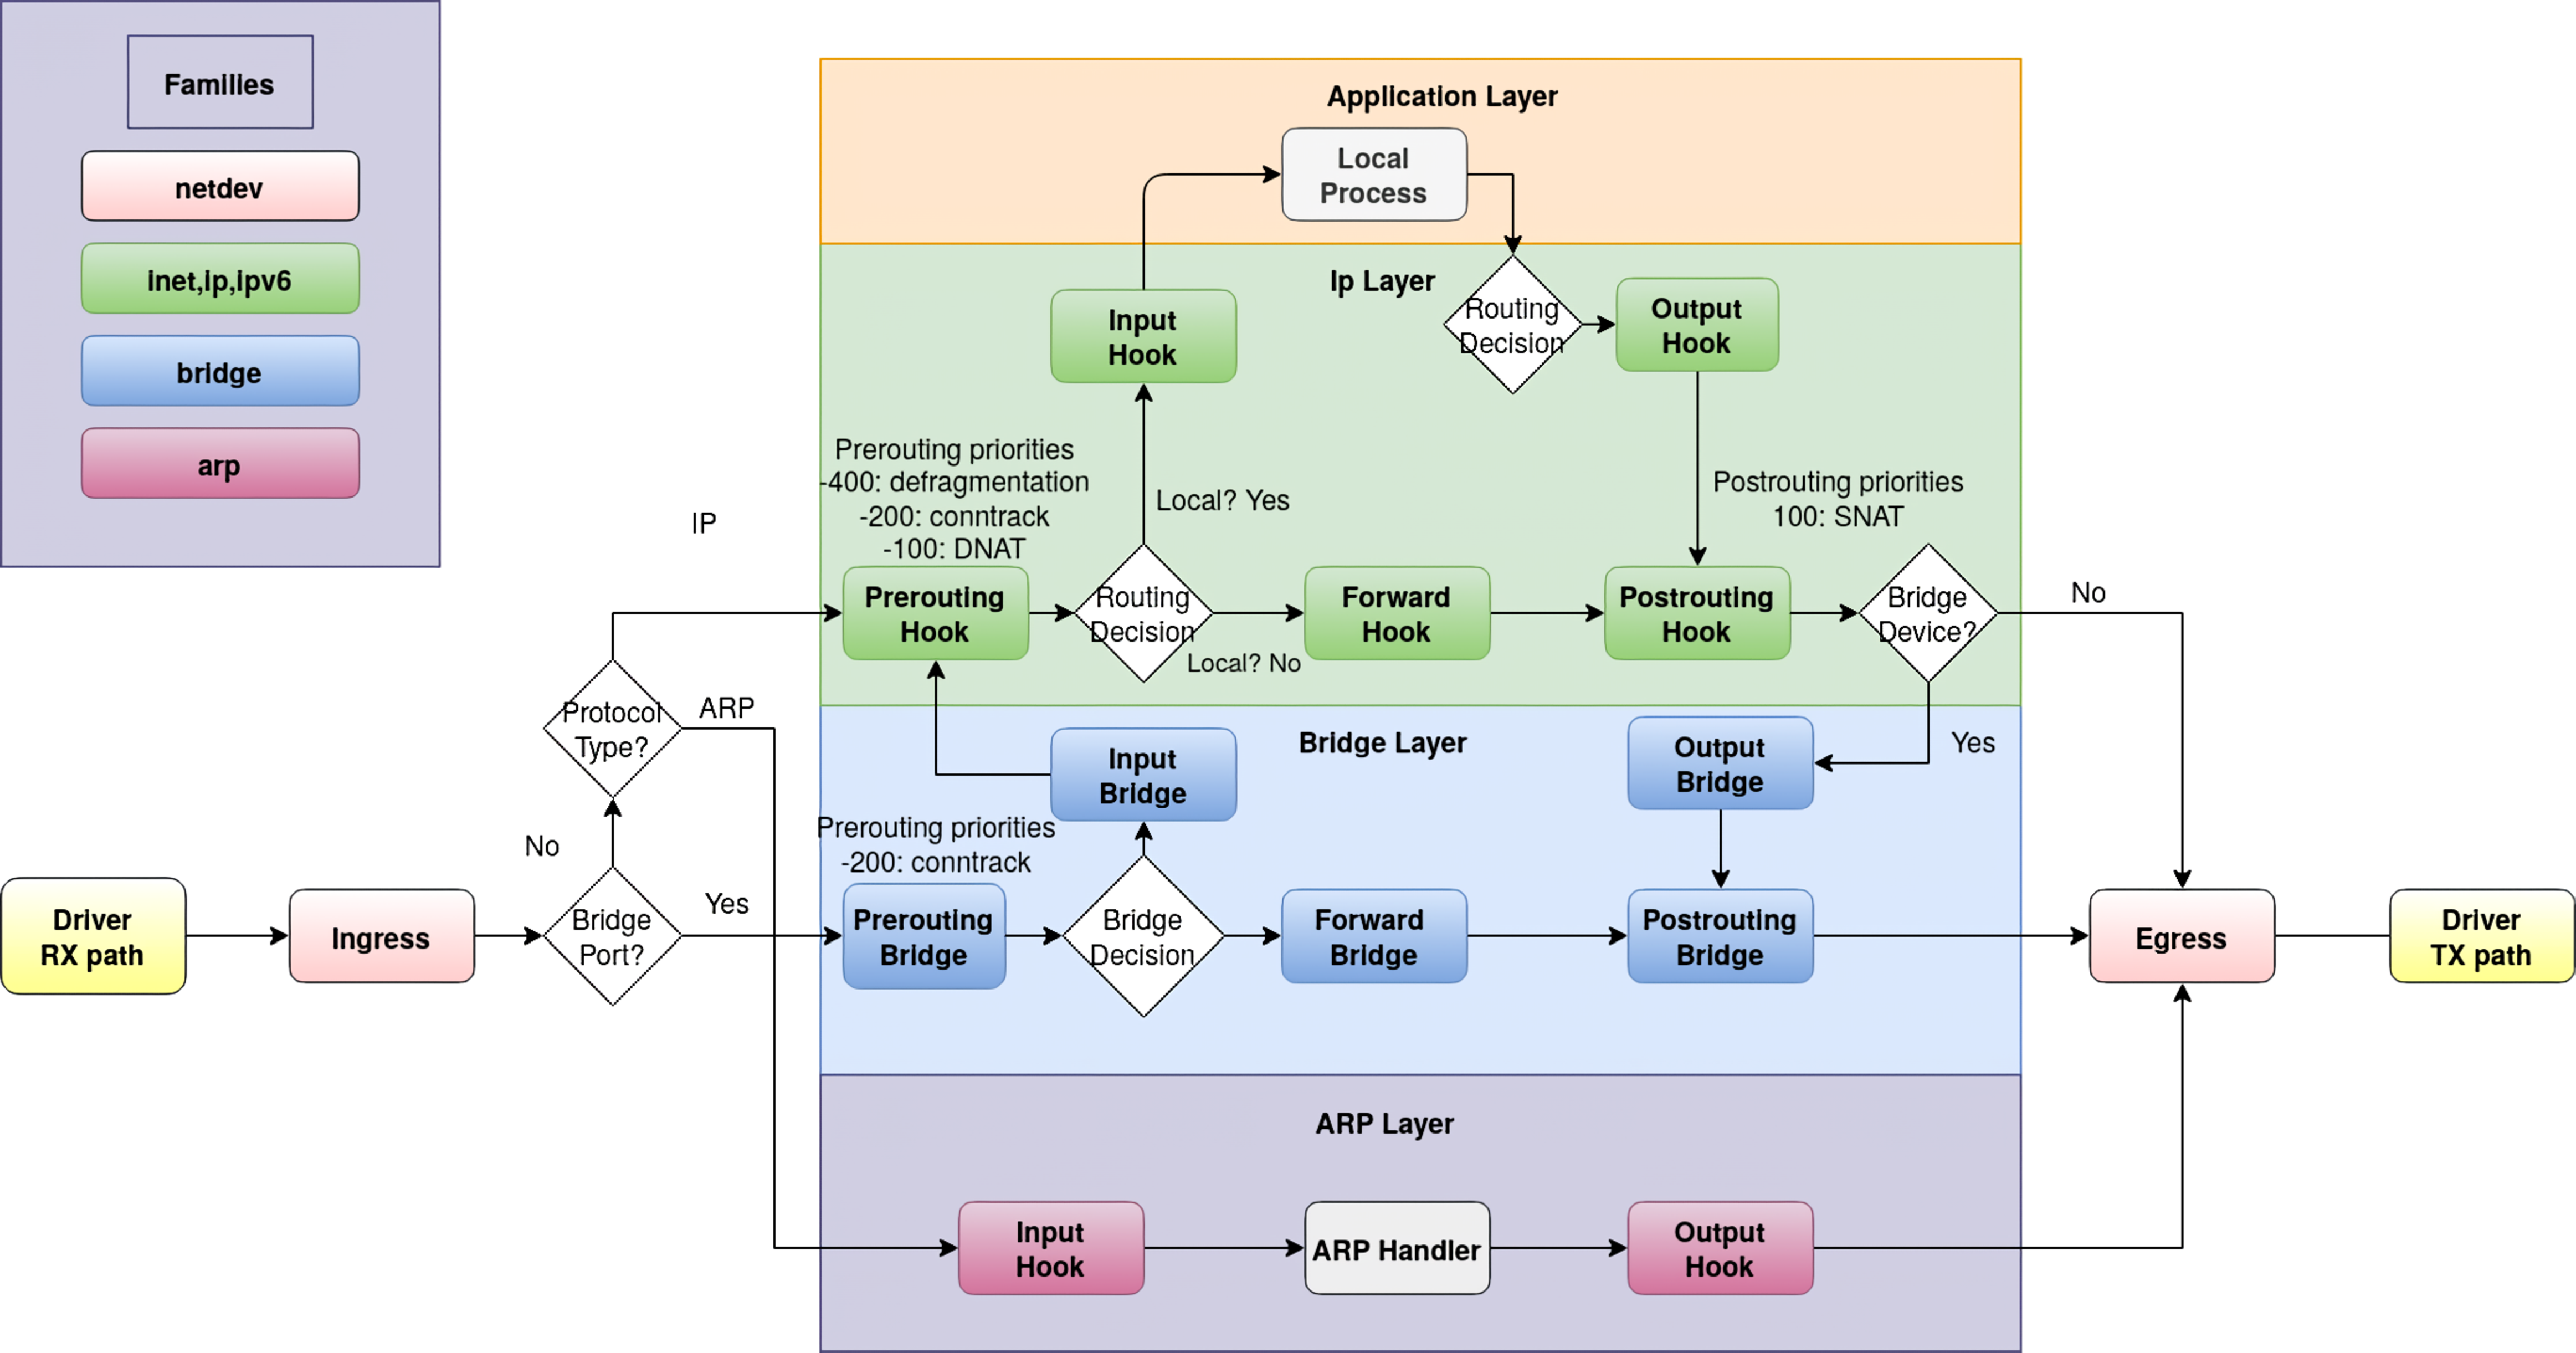
\includegraphics[width=0.95\linewidth]{img/nf-hooks.pdf}
    \caption{netfilter hook points (wiki.nftables.org より引用~\cite{nf-hooks})}
    \label{fig:nf-hooks}
\end{figure}

\section{SRv6 と SF としての netfilter 統合手法}
\label{section:netfilter-as-nf}
Linux netfilter と SRv6 を利用して SFC をデプロイすることは有用な手法であるように思えるが,実際には問題が存在する.
章~\ref*{section:linux-and-netfilter}で述べたように,Linux kernel には SRv6 の機能が実装されており,netfilter は SF アプリケーションの開発に有用である.
しかし,netfilter は SRH でカプセル化された内部のパケットに対して netfilter hook point を適用できない.
これは転送するパケットのソースアドレスを書き換える NAT 操作を SRv6 パケットの内部に適用しようとしても,SRH でカプセル化されているために通常のパケットと同じ操作では NAT を適用することができないからである.
つまり,一般的な IPv4 パケットに対して特定の操作を行うために実装された netfilter-based アプリケーションを SRv6 の内部 IPv4 パケットに対して適用する事はできない.

SRv6 に対応していない SF アプリケーションのことを,SR-unaware アプリケーションといい,対照的に SRv6 に対応している SF アプリケーションのことを SR-aware アプリケーションという.
SR-unaware アプリケーションを SRv6 環境で SF として利用する方法はいくつか存在する.以降では,3 つの手法について解説する.

\subsection*{アプリケーションの実装を変更する手法}
\label{sbsection:change-impl}
最も単純な方法は,アプリケーション自体の実装を変更し,SR-aware アプリケーションにすることである.
SERA~\cite{sera} は,Linux iptables に統合された SR-aware アプリケーションの実装である.
SERA は Linux iptables を拡張し,SRH のフィールドと iptables のルールをマッチさせて,ファイアウォール用のフィルタリングルールを適用する.
また,SERA は SRH でカプセル化された内部の IPv4 パケットに対してファイアウォールルールを適用する事もできる.
更に SERA は,SRv6 End ビヘイビアのように,パケットを次の SID に転送する機能も持つ.
しかし,SERA は iptables の拡張であるため,その他の netfilter-based アプリケーションを SR-aware にすることはできない.
SERA のような手法で netfilter-based アプリケーションを SR-aware にするためには,アプリケーション毎にその実装を変える必要がある.
また,SERA の採用した iptables を拡張するというデザインは,SERA に関連する SID を既存のルーティングインフラに統合することを困難にしている.
iptables 内のフィルタリングルールとして利用するための SID の情報は,\ref*{section:srv6}章で解説した layer-3 VPN の例とは異なり,既存のルーティングプロトコルを通じて広告することはできない.

\subsection*{SR-proxy を利用する手法}
\label{sbsection:use-sr-proxy}
もう 1 つの方法は,SR-proxy と呼ばれる手法を適用することである.
SR-Proxy の概念図を図~\ref*{fig:sr-proxy} として示す.
図~\ref*{fig:sr-proxy} において,Router-B が SR-proxy を適用するノードである.
Router-B は,Router-A から受信した SRv6 パケットの SRH を一度取り外し,その状態をキャッシュしておく.
Router-B は,取り外して得られた SRv6 の内部パケットを FW ノードへ送信する.
FW ノードが受信するパケットは SRH でカプセル化されてない一般的な IP パケットであるため,FW ノードは受信したパケットを一般的な IP パケットとして解釈し,FW サービスを適用する.
FW ノードは,FW サービスを適用したパケットを再び Router-B に送り返す.
Router-B は FW サービスから受け取った非 SRv6 パケットを,キャッシュしておいた SRH で再びカプセル化する.
Router-B は自身が再度カプセル化した SRv6 パケットを,次の転送先である Router-C へ送信する.

SR-Proxy を利用する方法は,汎用性が高い.
SR-Proxy を実行するノードが SRH を取り外して SF ノードにパケットを転送するため,SF アプリケーションは SRH の存在を意識する必要がない.
この手法であれば,iptables に限らず,あらゆる netfilter-based アプリケーションを SFC 中の SF として扱うことができる.

また,SR-Proxy は SRv6 のビヘイビアとしても提案されており~\cite{filsfils-spring-srv6-interop-02},End.AS や End.AD や End.AM と呼ばれるビヘイビアがそれに該当する.
これらは SRv6 ビヘイビアであるため,それら SID は IPv6 アドレスとして表現され,既存のルーティングプロトコルを使ってそれらの SID を広告することができる.
2024 年 1 月現在,End.AD や End.AM は Linux kernel のメインライン上では実装されておらず,これらの実装はワークインプログレス状態である.
Linux で動作する SR-Proxy として,SRv6 ビヘイビア以外の実装も提案されている~\cite{sfc-proxy-bpf,sfc-with-leg-vnf,afxdp-for-srv6}.

しかし,SR-Proxy を利用する方法には,SERA のような SR-aware アプリケーションには存在しないオーバーヘッドが存在する.
それは,SR-Proxy が一度 SRv6 パケットから SRH をデカプセル化する際に生じるオーバヘッド,一度外部ノードに転送し,SF 適用後に再度受信するオーバーヘッド,そして受信したパケットを再度同じ SRH でカプセル化するオーバーヘッドである.

また,SR-Proxy は根本的にネットワークにさらなる複雑さをもたらす.
SR-Proxy は SF から返されるパケットに付加する適切な SID リストを決定する必要がある.
SF から返される内部パケットは任意の宛先と送信元を持つ可能性があるため,SR プロキシが付けるべき SID リストは内部パケットによって異なる可能性がある.
つまり,SRプロキシは適切な SID リストを決定するための独自のメカニズムを実装する必要がある.
例えば,静的な SID リストをアタッチする End.AS か,プロキシの内部で状態をキャッシュする必要がある~\cite{sfc-proxy-bpf} .
さらに,SR プロキシをデプロイするためにはいくつかの問題が存在する.
例えば,特定の SR-Proxy タイプと共存できないサービスのタイプがあったり,サービスの有効性を検出する必要や SR-Proxy が送信する先の SF に関する SID 広告の問題など~\cite{draft-scexp}が既にインターネットドラフトとして挙げらている.

\begin{figure}[t]
    \centering
    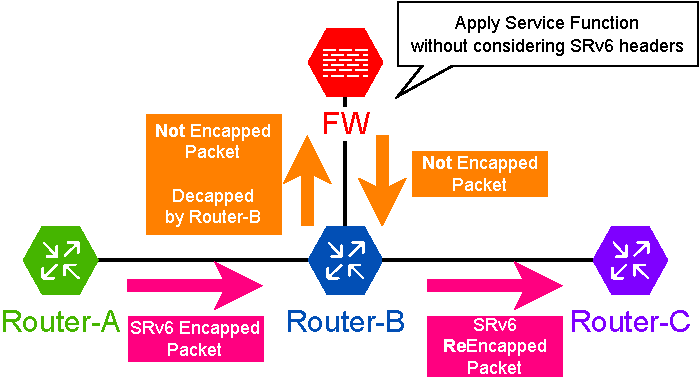
\includegraphics[width=0.95\linewidth]{img/SR-proxy.pdf}
    \caption{SR-proxy Architecture}
    \label{fig:sr-proxy}
\end{figure}

%%%
% \ref*{section:srv6}章で示した End.DT4 及び H.Encaps は,パケットをカプセル化,及びデカプセル化するビヘイビアである.
% 一方で,いくつかのビヘイビアのもつ機能はパケットのカプセル化,及びデカプセル化に限定されていない.
% SRv6 では,パケットに適用される NF (Network Function) も SID で表現可能である.
% NF がトランジットパケットに対して,segleft をデクリメントし,宛先 IPv6 アドレスを次の SID で更新する End ビヘイビアとしての動作をしながらネットワークサービスを適用する場合,その NF は SR-Aware ファンクションと呼ばれる.

% SR-Aware ファンクションと対照的に,従来の SR-unaware NF を SRv6 ベースの SFC に統合するための様々な方法論が提案されている.
% SR プロキシ~\cite{ietf-spring-sr-service-programming-08} は,SR-unaware NF を SRv6 ネットワークに接続するための重要なコンポーネントである.
% SR プロキシは ローカル SID 宛のパケットを受信し,SRH を持たないインナーパケットを関連する NF に渡した後,NF から返されたパケットに適切な SRH を再度付加し,次の SID にパケットを転送する.
% Linux における SR プロキシの実装もいくつか提案されている~\cite{sfc-proxy-bpf,sfc-with-leg-vnf,afxdp-for-srv6}.
% しかし,SR プロキシは根本的にネットワークにさらなる複雑さをもたらす.
% 例えば,SR プロキシは NF から返されるパケットに付加する適切な SID リストを決定する必要がある.
% 内部パケットは任意の宛先と送信元を持つ可能性があり,そのため SR プロキシが付けるべき SID リストは内部パケットによって異なる可能性がある.
% SRプロキシは,適切なSIDリストを決定するための独自のメカニズムを実装する必要がある.
% 例えば,静的な SID リストをアタッチする End.AS か,プロキシの内部で状態をキャッシュする必要がある~\cite{sfc-proxy-bpf} .
% さらに,SR プロキシをデプロイするためにはいくつかの問題が存在する.
% 例えば特定の SR プロキシタイプと共存できないサービスのタイプ,サービスの有効性の検出,SR プロキシの背後のサービスに対する SID 広告の問題など~\cite{draft-scexp}が既にインターネットドラフトとして挙げらている.


% \textbf{[この段落では End.eBPF について述べる]}
% \begin{itemize}
%     \item eBFP とはなにか
%     \begin{itemize}
%         \item eBPF を使って NF を作ることができる 
%         \item 最近では LKM に変わって Linux kernel を拡張する方法としての側面に注目が集まっている
%         \item eBPF は Virtual Machine で動作するものの Linux kernel に依存する機能も多い
%     \end{itemize}
%     \item End.eBPF とはなにか
%     \item eBPF に対して,本研究では netfilter を NF に統合することを目的としている
%     \begin{itemize}
%         \item ここで Linux kernel に依存する End ビヘイビアを提案することの妥当性を述べる
%     \end{itemize}
% \end{itemize}

\section{問題提起}
\label{section:prob}
現在,Linux の持つ SRv6・IPv6 ルーティングインフラストラクチャを活用しながら Linux カーネルに実装されている netfilter という多機能なパケット処理機能 を NF として利用する手法は,確立されていない.
現在提案されている手法では,Linux の持つ IPv6 ルーティングインフラストラクチャを活用した SR-aware アプリケーションをシンプルに汎用的に実現することは難しい.
また,Linux カーネルには netfilter という多機能なパケット処理機能が実装されているものの,SRv6 上で netfilter を直接 NF として扱う方法も確立されていない.
SRv6 は SF を SID として表すことで SFC を実現可能なアーキテクチャであるものの,SID として表現された SRv6 上のノードとしての SF と,実際のアプリケーションとしての SF を統合するの方法は自明ではない.
セクション~\ref*{sbsection:use-sr-proxy}で述べた SR-Proxy を利用する方法では,SR プロキシを導入することで生まれるオーバヘッドや運用上の問題が指摘されている.
また,SRH でカプセル化されているパケットに対して,パケットをカプセル化したまま netfilter 自体を適用する手法も確立されていない.
本論文では,Linux netfilter を SRv6 を使って構築された SFC 上の SF として活用するための手法を提案する.
